\documentclass[conference]{IEEEtran}
\IEEEoverridecommandlockouts
% The preceding line is only needed to identify funding in the first footnote. If that is unneeded, please comment it out.
\usepackage{amsmath,amssymb,amsfonts}
\usepackage{algorithmic}
\usepackage{graphicx}
\usepackage{xcolor}
\usepackage{listings}
\usepackage{array}
\usepackage{qtree}
\usepackage{spreadtab}
\usepackage{tabularx}
\setlength\extrarowheight{3pt}

% Beramono font.

\usepackage{tgpagella}        
\usepackage[scaled=0.85]{beramono} 
\usepackage[T1]{fontenc}     
\usepackage{makecell} 

\renewcommand\theadfont{\bfseries}
\renewcommand\theadgape{\Gape[4pt]}
\renewcommand\cellgape{\Gape[4pt]}
\newcommand{\astname}{GAST}

\newcommand{\toolname}{GT}

\newcommand{\astbuilder}{\textit{\astname{} Builder}}

\newcommand{\implangs}{Java, PHP, Python and JavaScript}
\newcommand{\converter}{\textit{AST Converter}}
\newcommand{\taintanalyzer}{\textit{Taint Analyzer}}

\definecolor{codegray}{rgb}{0.5,0.5,0.5}

\lstset{
  extendedchars=false,
  basicstyle=\ttfamily\small,
  frame=top,frame=bottom,
  captionpos=b, numbers=left,xleftmargin=2em,framexleftmargin=2em,
  numberstyle=\scriptsize \color{codegray},
}

\def\BibTeX{{\rm B\kern-.05em{\sc i\kern-.025em b}\kern-.08em
    T\kern-.1667em\lower.7ex\hbox{E}\kern-.125emX}}
\begin{document}

\title{Virtual Static Security Analyzer for Web Applications}

\author{\IEEEauthorblockN{Mihail Brinza}
\IEEEauthorblockA{\textit{Instituto Superior Técnico}\\
Lisbon, Portugal \\
mihail.brinza@tecnico.ulisboa.pt}
\and
\IEEEauthorblockN{Miguel Pupo Correia}
\IEEEauthorblockA{\textit{Instituto Superior Técnico}\\
Lisbon, Portugal \\
miguel.p.correia@tecnico.ulisboa.pt}
\and
\IEEEauthorblockN{João Pereira}
\IEEEauthorblockA{\textit{Instituto Superior Técnico}\\
Lisbon, Portugal \\
joao.d.pereira@tecnico.ulisboa.pt}
}


\maketitle

\begin{abstract}
In the past decades web applications have been popular victims of injection attacks such as SQL injection or cross-site scripting. In order to prevent these attacks, we need automatic vulnerability detection tools. However, modern existing tools are complex, consist of thousands of lines of code, and are often bound to a single language. This complexity makes them hard to understand and to port to a new language. 


To reduce the complexity of current static analyzers, we propose a new solution that supports the addition of new languages without much effort. In order to achieve this, our solution does not analyze the source code AST directly, instead, it traverses the source code AST and builds a generic AST (\astname{}) from it. Then, we analyze the \astname{} to find vulnerabilities. This way we can decouple the analysis and the source code parsing. Furthermore, \astname{} is just an abstraction that only represents what is needed to perform taint analysis, ignoring the rest. To add support for a new language we just need to generate a parser using ANTLR4 \cite{antlr4book} and write a converter for that AST, which is usually less than 110 lines of code. 

We implemented a tool called GT with this approach. The tool supports \implangs{}, and was tested against several web applications written in the same languages.
\end{abstract}
\begin{IEEEkeywords}
Security, Static Analysis, Taint Analysis, Antlr4, Information Flow
\end{IEEEkeywords}


\section{Introduction}
In the past couple of decades, research on web security and bug finding tools have seen a big increase. This is due to the fact that software vulnerabilities can have devastating effects on companies and/or its clients \cite{telang2007empirical}. In 2017, hackers have compromised the sensitive information of 145 million American customers from Equifax, one of the three major consumer credit reporting agencies in the U.S.A, leading to hundreds of millions of dollars of loss to the company \cite{equifax}.

Web applications are popular victims of security attacks since they accept user input, which can be malicious, and incorporate it into dynamically generated code. 
For example, a user may have to fill a form, post a comment, or submit a username and a password for authentication. 
The application then takes this user-provided input and inserts it into a dynamically generated program in another language (e.g., a new client-side script, or an SQL or JavaScript query to a back-end database). If the user input reaches these scripts/queries without first being validated and sanitized, then there is probably a vulnerability.

\textit{Code injection attacks} such as SQL injection or cross-site scripting were considered the top security problem in 2017 by OWASP \cite{OWASP}. These attacks occur when a malicious user manages to inject his code into dynamically generated scripts/queries, usually by adding meta-characters to the input. By doing this, an attacker could change the behavior of the application, steal data, compromise database integrity and/or bypass authentication and access control, violating system correctness, security, and privacy properties.

Injection vulnerabilities are caused mainly by poor user input sanitization, the use of languages where it is easy to write insecure code (e.g., PHP, C) and programmers that do not have much knowledge about software security \cite{jain2011review}.

In order to detect and prevent injection attacks, we need automatic detection mechanisms.
While researchers have tried many approaches over the past decades, (e.g., static and dynamic taint analysis, symbolic execution, etc.) the dominant trend is towards increasingly complex tools. However, the more complex a tool is, the worse it scales, the harder it is to maintain and understand, and the more assumptions it makes, limiting the programs it can analyze. 

One big problem of the increasing complexity in vulnerability detection tools is that most of the times they are not \textit{portable}\footnote{In this paper we use the term \textit{portable} to refer to the approaches that either support different languages or to which it is easy to add support for a new one.}. Although most of the programming languages we use nowadays to build web applications have a lot of similarities between them, vulnerability detection tools still seem to struggle when it comes to supporting more than one language. Many of them are wedded to a specific language \cite{diglossia,phpapis,jovanovic2006pixy, arzt2014flowdroid,nunes2015phpsafe,wassermann2008static, dahse2014simulation,livshits2005finding}, a specific compiled code \cite{dytan,taintcheck,dt++} (e.g., x86 binary, bytecode) or they depend on modified runtime engines \cite{diglossia,phosphor}. To port one of these tools to another language basically requires to implement it again from scratch. 

Since there is a wide range of languages available to build web applications, the lack of portability of the detection tools can be considered a problem and a limitation. However, there are some approaches that solve this issue to some degree which we discuss in section \ref{relatedwork}. Also, the tools that are specific to a language have the advantage of being able of taking into account every feature of that specific language, which in theory could lead to a more precise analysis.

In this paper we present a new static taint analysis approach, alongside a tool we implemented with this approach, called {\it Generic Taint analyzer} (GT), that aims to solve the problem of portability while being context-sensitive and keeping low rates of false positives and negatives. Our solution is not bound to a specific language and can be extended to support a new language with a relatively small amount of work and lines of code. 
Traditional static taint analyzers parse the code and then analyze the resulting abstract syntax tree (AST). The nodes that the AST consists of are specific to the parsed language, making the tools bound to that language. However, most of the languages we use nowadays to build web applications are similar. Languages usually consist of classes, attributes, functions or methods, statements, expressions, etc... Even between languages such as PHP and Java, that are apparently very different, we find many of these structural similarities. Based on this fact, our approach converts the source code AST to a simple, generic abstract syntax tree (\astname{}) that can represent a large set of languages used in web applications. More importantly, the \astname{} does not represent all the details of a language. Instead, it only has the aspects that are actually used in the analysis. This way, we  use the same code to find vulnerabilities, regardless of the language being analyzed. The \astname{} allows us to keep the source code parsing and the analysis decoupled.

Due to the \astname{}, the analysis is divided into three main steps, where each one uses a different module (\textit{parser, converter, analyzer}):

\begin{enumerate}
    \item Use a \textit{parser} specific to the language to get the source code AST
    \item Convert the source code AST to a \astname{} using a specific \textit{converter}

    \item Run an \textit{analyzer} on the \astname{} to find vulnerabilities. In our case, the \textit{analyzer} is a static taint analyzer
\end{enumerate}

The only modules that are bound to each language are the \textit{parser} and the \textit{converter} (which converts the source code AST to the \astname{}). Since parsing several different languages is a complex problem, we use ANTLR4 (ANother Tool for Language Recognition) to generate the \textit{parser}, parse the source code and build the AST. ANTLR4 is a parser generator with a big community that provides grammars under the MIT license for virtually any language. This way, when adding support for a new language we only need to generate a new \textit{parser} with ANTLR4 and program a new \textit{converter}, which in our opinion requires a small amount of work. While implementing the \toolname{} tool, we started by adding support for PHP and Java. Later, we extended the tool to support JavaScript and Python. Converters for \implangs{} are all less than 110 lines of code each. 

The main contributions of this paper are: (1) an approach for improving portability of static security analyzers by converting the source code AST to a \astname{}; (2) a open-source tool that implements this approach written in Java for applications written in \implangs{}.



\section{Input Validation Vulnerabilities}
This section briefly presents a list of vulnerabilities considered in this work. We can divide them in four categories \cite{iberia} - \textit{query manipulation, client-side injection, file and path injection} and \textit{command injection}. The main problem of all these vulnerabilities lies in the improper validation of user input. Our work focuses on this kind of vulnerability.

\subsection{Query Manipulation}
These vulnerabilities are associated with the construction of queries or filters that are executed by some other engine (e.g., a database management system). If the query is constructed with unsanitized inputs, then it is possible to modify the normal behavior. 

All vulnerabilities in this category can be prevented by sanitizing user input, so it does not contain meta-characters that can alter the behavior of the engine:

\subsubsection{SQL Injection} vulnerability caused by the use of string building functions to create SQL queries. An attack consists of mixing normal characters with meta-characters. In the example of listing \ref{phpsql}, a malicious user can provide a username \texttt{"admin' ---"} causing the query to execute without the need of a password. 

\begin{lstlisting}[language=PHP,
    showstringspaces=false,
    caption={PHP code vulnerable to SQL Injection},
    label=phpsql]
$name = $_GET['username'];
$pass = $_GET['password'];
$query = "SELECT * FROM users 
    WHERE name='$name' AND password='$pass'"; 
$result = mysql_query($query);
\end{lstlisting}


\subsubsection{NoSQL Injection} Similarly to relational databases, non-relational are also vulnerable to injection attacks. 

\subsubsection{XPath Injection} This vulnerability is very similar to SQL Injection, but in this case, data is injected in XML documents, which are often used to store data or configurations. To prevent this vulnerability, it is enough to check if the input contains malicious characters.

\subsubsection{LDAP Injection} (Lightweight Directory Access Protocol) Injection is also exploited by providing meta-characters to string-building functions. LDAP Injection attacks aim to modify the structure of the filter and retrieve data from a directory.

\subsection{Client-Side Injection}
The vulnerabilities in this category allow an attacker to execute malicious code in the victim's browser. This kind of attack is not against the application itself but against the user and can be prevented by either sanitizing or encoding the input.
\subsubsection{Cross-site scripting (XSS)}
There are three types of XSS attacks: reflected or non-persistent, stored or persistent and DOM-based. In this paper we only consider the first two types.

A program vulnerable to reflected XSS can have a single line, \textit{"echo \$\_GET['user'];"} 
The attack consists of convincing the user to click on a link to the web application with a malicious script which will be reflected by the \textit{echo} instruction. (e.g., \textit{www.a.pt?user=<script>*malicious code*</script>}).

A stored XSS consists of two steps: first, the attacker inserts a malicious script in the server, then later, the server returns that script to one or more users.

\subsubsection{Header injection} allows an attacker to break the HTTP  response with \textit{"\textbackslash n"} and \textit{"\textbackslash r"}. This allows the attacker to inject malicious code in headers or even a new HTTP  response. It can be avoided by sanitizing these characters.

\subsubsection{Email injection} Very similar to Header Injection, it has the goal to manipulate email components (e.g., sender, destination, message) by injecting the line termination character. In this case, sanitizing the input solves the problem as well.

\subsection{File and Path Injection} This category consists of vulnerabilities where the user can control the path or the URL of the file included. Thus allowing him to inject malicious files (\textit{Remote file inclusion}) or read arbitrary files from the server (\textit{Directory/Path traversal}).


\subsection{OS Command injection} 
This category consists of vulnerabilities where the user can control the input to functions that execute OS commands (e.g., \textit{shell\_exec} in PHP). Allowing the attacker to execute arbitrary code in the server.






\section{The \toolname{} tool}
\label{solution}
In this section we explain in-depth our approach at solving the complex problem of developing a portable static taint analyzer. Our solution, besides being portable, also aims to be able to perform a context-aware analysis, being as sound and complete as possible.

As stated before, static analyzers are most often bound to a single language and depend on every detail of that language. However, there are a lot of similarities between programming languages, and our approach explores just that. If we take a look at the top trending languages in 2020, ranked by IEEE Spectrum \cite{cass2020top}, used to build web applications, we can divide them in two categories:

\begin{enumerate}
    \item Dynamically typed - Languages that do not check or enforce type-safety at compile-time \cite{tratt2009dynamically}. Instead, type-checking is done during runtime (e.g., Python, JavaScript, PHP and Ruby).
    \item Statically typed - Type checking is done at compile-time. (e.g., Java, C\#, GO and Dart).
\end{enumerate}


The languages from each category have many similarities between them. Take for instance JavaScript and PHP, which are very common on web applications. Both of them are object-oriented, have methods, functions, attributes, variables, expressions, etc... Even the \textit{control flow statements} are practically the same (e.g., \textit{if, switch, while, for, do while} etc.). Furthermore, the data flow is almost identical, using assignments. 

Now, if we compare Java and C\# the same is true. Moreover, even comparing languages between categories (e.g., Java and PHP) we see that many of their features overlap. The main difference is that we know the types when analyzing the source code. So from our studies, we found out that when it comes to static taint analysis we can abstract almost any web programming language. 

With this in mind, our approach introduces a new way of building static analyzers, which consists of having a simple, generic AST (\astname{}) that can represent the structure of the source code of a large set of languages found in web applications. The \astname{}, similarly to the micro-grammars approach \cite{microgrammars}, does not depend on every detail of the languages. Instead, it only represents what is absolutely needed to perform a data flow analysis (in our case, static taint analysis). Section \ref{genericast} explains the abstractions that were made to build the \astname{}.

With the addition of the \astname{}, our analysis gains an extra step comparing to traditional tools. Usually, analyzing a program consists of first parsing the source code and then traversing the resulting AST to find vulnerabilities. By contrast, our approach adds a new, additional step, which consists of converting the source code AST to a \astname{}. Then, we perform the taint analysis on the \astname{} to detect vulnerabilities in the code. This way, the module that performs the taint analysis is completely independent of the language being analyzed. 

Next, we describe the architecture and data flow of \toolname{}. Then, we present the  structure of the \astname{} and how to build it. Finally, we discuss the features of our taint analysis and the compromises and choices that were made.

\subsection{Architecture and Data Flow}

In order to implement a tool that can support several languages simultaneously, we need a decoupled and modular architecture. The architecture of \toolname{}, represented in figure \ref{architecture}, consists mainly of four modules: \textit{Parser}, \textit{AST Converter}, \astbuilder{} and \textit{Taint Analyzer}.


\subsubsection{Parser} takes as input the source code and produces a source code AST, specific to the language. This module is language-dependent, meaning that every time we add a new language, we need a new parser for that language. Since parsing a full-blown language is a complex task, we delegate it to ANTLR4, which is a widely used parser generator that uses \textit{LL} for parsing \cite{antlr4book}. ANTRL4 has a big community and provides grammars under the MIT license for virtually any language. This way, thanks to ANTRL4, our parsers consist simply of generated code. Furthermore, ANTRL4 also generates tree walkers, which we use to traverse the AST.

\subsubsection{AST Converter} traverses the source code AST using the generated tree walker and raises events to the \astbuilder{} (e.g., entering and exiting class, methods or functions declarations). These events allow the \astbuilder{} to create the \astname{}. This module is the only one needed to program whenever adding support for a new language.

\subsubsection{\astname{} Builder} reacts to the events from the \textit{AST Converter} and internally builds the \astname{}. Section \ref{buildgenericast} shows more in-depth the process of building the \astname{}. 

\subsubsection{Taint Analyzer} module that takes as input the \astname{} from the \astbuilder{} and a configuration file where we can specify the value of several parameters, such as:
\begin{itemize}
    \item Sensitive functions - functions that when called with \textit{tainted} arguments may result in a vulnerability (e.g., \textit{mysql\_query} in PHP)
    \item Sanitization functions - functions that perform input sanitization and whose return value is always \textit{untainted} (e.g., \textit{mysqli\_real\_escape\_string} in PHP)
    \item Entry points - the function which is invoked by the server when the user makes a request. We also specify which arguments of the entry point function are \textit{tainted}
\end{itemize}

After traversing the \astname{}, \toolname{} produces a vulnerability report. 

\begin{figure}[h]
    \centering
    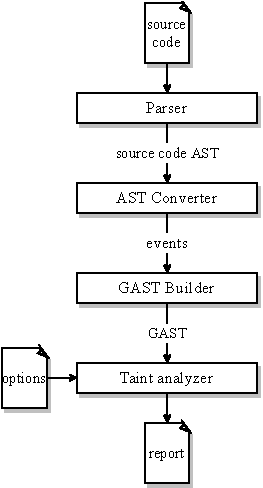
\includegraphics[width =0.5\linewidth]{images/yasat-architecture.pdf}
    \caption{\toolname{} - data flow and architecture overview} 
    \label{architecture}
\end{figure}

\subsection{\astname{}}
\label{genericast}
Similarly to the micro-grammars solution \cite{microgrammars}, the \astname{} aims to be an intermediate structure that does not depend on every detail of any language. Instead, it abstracts most of the complexity by using generic statements. Each generic statement has a correspondence with a concrete statement of almost any programming language. In this section we describe the structure of the \astname{} by presenting every element that can be part of it. 

\subsubsection{Constant} comprises \textit{strings}, \textit{integers}, \textit{floats}, \textit{null} values etc. Basically, everything that is directly hardcoded in the source code is considered a constant. Since this element never changes, it is impossible to be \textit{tainted}.
 
\subsubsection{Variable} as the name says, it represents the variables in the code. Contains the name of the variable, and if the language is statically typed, it also contains the type of the variable. It can become \textit{tainted} through assignments.

\subsubsection{Attribute} represents an attribute in a class. It has a name and a type. Also, it can be \textit{tainted}.

\subsubsection{Parameter} represents a function or a method parameter. It can be \textit{tainted} if it is the parameter of the entry point function, or if the argument passed to a function is \textit{tainted}.

\subsubsection{Expression} represents a generic abstraction of any expression (e.g., arithmetic, logical, bitwise, comparison etc.). It consists of a list of expressions.
Take for instance the listing \ref{javaexpression} where to each variable, \textit{a, b, c} we assign an expression. In our representation, all these expressions are equal. They all consist of an expression containing two members: a variable named \textit{"x"} and a constant with value \textit{"5"}. This allows us to abstract any operator due to the fact that in data flow analysis, operators (except the assignment operators) do not influence \textit{taint} propagation. For instance, if the variable \textit{x} in listing \ref{javaexpression} is \textit{tainted}, then, all variables will be \textit{tainted}, regardless of their operator.


Since an expression consists only of a list of other expressions, the \textit{taint} propagation is a result of a logical OR of all elements in the expression. Meaning that if any element in the list is \textit{tainted}, the whole expression is marked as \textit{tainted}. 

\begin{lstlisting}[language=Java,
    showstringspaces=false,
    caption={Expression assignment examples},
    label=javaexpression]
boolean a = x == 5;
int b = x + 5;
int c = x * 5;
\end{lstlisting}

\subsubsection{Function Call} this is a subtype of \textit{expression} with the difference that it has a name, referencing the function it is invoking. The arguments are just a list of expressions that can contain anything. For instance, the function call \textit{executeQuery(getQuery("name"))} is named \textit{executeQuery} and has as argument another function call named \textit{getQuery}. The latter having as argument a constant with value \textit{"name"}.

A function call is considered \textit{tainted} if any of the following conditions is true: 
\begin{itemize}
    \item the called function is in the source code and it returns a \textit{tainted} value
    \item the called function is in a library and any of its arguments is \textit{tainted}
\end{itemize}

This element also represents method calls that do not have an object as a source (e.g., methods from the same class or any superclass that are not preceded by the keywords \textit{this} or \textit{super} in Java).


\subsubsection{Assignment} statement that represents, as the name indicates, an assignment. Consists of two expressions, one on the left-hand side and another on the right-hand side. It is the main way of propagating \textit{taint} marks. Whenever the expression assigned on the right is evaluated as \textit{tainted}, the mark is also propagated to the expression on the left. Usually, the expression on the left-hand side is just a variable. Listing \ref{javaexpression} contains examples of assignment statements.


\subsubsection{Return} statement that represents the end of the data flow for a path. The returned value is represented by an \textit{expression}, which can be \textit{tainted}.


\subsubsection{Throw} statement very similar to the return statement. The only difference is that when a return statement is found in the callee function, the data flow is transferred to the caller function. Whilst in the case of a throw statement, the data flow is transferred to a catch block. The thrown expression can be \textit{tainted}.


\subsubsection{Method Call} this element represents method calls. It consists of a source, which can be an object or a class (if the method is static). Listing \ref{methodcall} shows examples of method calls where the source is an object and a class respectively. A method call is \textit{tainted} if any of the following conditions is true:

\begin{itemize}
    \item the method is not in the analyzed code and the source is \textit{tainted}
    \item the method is in the source code and returns a \textit{tainted} value
\end{itemize}

\begin{lstlisting}[language=Java,
    showstringspaces=false,
    caption={Method call examples},
    label=methodcall]
context.getUsers();
MyClass.myStaticMethod();
\end{lstlisting}


\subsubsection{New} expression that represents an object creation. It works mostly as a function call to the constructor. In most languages, the constructor has the same name as the class. But in some languages, the name of the constructor is different from the name of the class (e.g., PHP, Python). For these cases, we keep a configuration file with the names. For instance, \textit{new Foo()} in PHP would result in the call of \textit{\_\_construct()} function of the class \textit{Foo}.

\subsubsection{Attribute access} represents a direct access to an object attribute (e.g., \textit{context.myProperty}).


\subsubsection{Code block} represents a block of code. Consists of a list of statements. Listing \ref{javaexpression} is an example of a code block with three statements.

\subsubsection{Conditional statement} this element represents loops (e.g., \textit{for, while, do while} etc.). Consists of a code block and a condition, which is an \textit{expression}.

\subsubsection{Try Catch} statement composed of a \textit{try} code block, a list of \textit{catch} code blocks and a \textit{finally} code block. 


\subsubsection{If} statement that represents control flow statements (e.g., \textit{if-else, if-elseif-else} and \textit{switch}). Each option in the control flow has its own code block (e.g., \textit{if-else} has two code blocks - one for \textit{if} and another for the \textit{else}).

\subsubsection{Function} element that represents a method or a function. It has a name, a return type, a list of parameters and a code block.

\subsubsection{Class} element that represents a class. It has a name, a list of attributes and a list of methods. Furthermore, it can have a superclass.

\subsubsection{File} this is the root element of any \astname{}. It has a code block (for languages like PHP or JavaScript), a list of classes, a list of functions and a list of imported files (used to trace calls to imported function).




One important note to keep in mind is that not every language will use every feature from the \astname{}. For instance, the file element can have statements directly in the root block. Now, this is a feature that it is only used by languages such as PHP and JavaScript. By contrast, Java and C\# do not allow code outside classes, so they do not make use of this feature. 

\subsection{Building the \astname{}}
\label{buildgenericast}


In order to build the \astname{}, we first parse the source code using a parser generated by ANTLR4 to obtain the source code AST. Then, we convert the AST to the \astname{} representation. To do this, we use a tree walker also generated by ANTLR4. The tree walker, which conceptually is a visitor, traverses every node of the AST and for each node it invokes a function when it enters or exits that node. So, in order to convert the AST to \astname{} we need to override some of these methods in the \converter{} to pass state to the \astbuilder{}. This is due to the fact that the \astbuilder{} keeps the current context in a stack and these methods indicate what is the new context to push and when to pop it. This way the \converter{} is just a class that overrides a set of methods from the generated tree walker. 

Listing \ref{funccallconvertexample} shows part of the PHP \converter{}. In the example, we override two methods from the generated tree walker. The first method is invoked when the tree walker enters a \textit{Func} node and the second when it exits the same node. So, when the tree walker reaches a \textit{Func} node, it invokes the method \textit{enterFunc} from the \converter{}. The latter then invokes a method from the \astbuilder{} that pushes the function element to the stack. This way, the \astbuilder{} is able to keep track of the context. For instance, if the tree walker encounters a \textit{Parameter} node while in the \textit{Func} node, the parameter would be added to the element on the top of the stack, which in this case would be a function. The function is then popped from the stack when tree walker exits the \textit{Func} node, invoking the method \textit{exitFunc} which calls a method from the \astbuilder{} that pops the function (line 8). 

\begin{lstlisting}[language=Java,
    showstringspaces=false,
    caption={Function declaration example},
    label=funccallconvertexample, float]
@Override
public void enterFunc(FuncContext ctx) {
    gastBuilder.addFunction(ctx, ctx.name());
}

@Override
public void exitFunc(FuncContext ctx) {
    gastBuilder.exitFunctionOrMethodDeclaration();
}
\end{lstlisting}

One important note is that we only push to the stack statements (e.g., functions, classes, assignments, conditional statements, etc.), which are nodes in the AST, while elements such as variables, constants or parameters are not pushed. This is due to the fact that they represent leaves in the AST, so they would be pushed and popped right away. This simplification allows us to override less methods from the tree walker when writing the \converter{} (e.g., we do not need to override \textit{exitVariable}).


Let us now consider listing \ref{assignmentconvertexample} where line 1 corresponds to the assignment being built and lines 3-9 to the sequence of calls made by the \converter{} to the \astbuilder{}. Due to lack of space, the signatures of the overridden methods are omitted. When the tree walker enters the assignment, the \converter{} calls a method that adds an assignment to the stack (line 3). Next, it enters a variable and since the assignment is on the top of the stack, the variable becomes the left side of the assignment (line 4). Then, the tree walker enters the expression \textit{"x == 5"} and the \converter{} calls a method that adds an expression to the stack (line 5). After that, it enters a variable and later a constant, which will both be added to the expression, since it is the top of the stack (lines 6, 7). Finally, the tree walker first exits the expression and then the assignment, calling \textit{exitStatementOrExpression} twice (lines 8, 9). Figure \ref{tree} shows the \astname{} representation of the assignment.
\begin{figure}[ht]

    \Tree[.Assignment 
    [.\textit{left} [.Variable [.\textit{name} a ] [.\textit{type} boolean ] ]]
    [.\textit{right} [.Expression [.\textit{members}  
        [.Variable [.\textit{name} x ] [.\textit{type} int ] ]
        [.Constant [.\textit{value} 5 ]]
        ]]] ]

    \caption{\astname{} resulting from executing listing \ref{assignmentconvertexample}}\label{tree}
\end{figure}

\begin{lstlisting}[language=Java,
    showstringspaces=false,
    caption={Assignment build call sequence},
    label=assignmentconvertexample]
boolean a = x == 5;
    
gastBuilder.addAssignment(ctx);
gastBuilder.addVariable(ctx.VarName());
gastBuilder.addExpression(ctx);
gastBuilder.addVariable(ctx.VarName());
gastBuilder.addConstant(ctx.getText());
gastBuilder.exitStatementOrExpression();
gastBuilder.exitStatementOrExpression();
\end{lstlisting}

Converting the AST is as simple as identifying the methods needed to override from the generated tree walker, and then call the methods from the \astbuilder{}.
For example, the \converter{} for PHP has 67 lines of code (counting only statements), and from these 67 statements, there are 29 that are different, meaning that a lot of the methods invoked are the same (e.g., \textit{exitStatementOrExpression} is invoked 23 times). 


\subsection{Analysis features}

Our approach is to use a context-aware static taint analysis to find all potential security vulnerabilities. To be able to statically find vulnerabilities, it is necessary to know what \textit{objects} each variable may refer to, a general problem known as \textit{pointer}, \textit{points-to} or \textit{alias analysis}\cite{sridharan2013alias}. Also, the tool must perform a \textit{path aware} \textit{taint} propagation. Furthermore, it must be able to detect function/method calls between different files.

Next, we discuss the importance of the \textit{alias analysis}. Then, we present our solution to a \textit{path aware} analysis and the method \toolname{} uses to find function/method calls from different files. Finally, we describe our approach to handle loops.

\subsubsection{Pointer information} to illustrate the importance of pointer information, consider the example from listing \ref{pointer}. Assume that \textit{param} is tainted and that \textit{executeQuery} is a sensitive function. In this example, a more conservative approach may assume that \textit{buf1} and \textit{buf2} may reference the same object, thus marking both calls to \textit{executeQuery} as tainted. Instead, \toolname{} traces the data flow through assignments made in each execution path. Thus, being able to identify that line 9 is a safe call and line 13 is a vulnerability.


\begin{lstlisting}[
    language=Java,
    showstringspaces=false,
    caption={Taint propagation example},
    label=pointer, float] 
String param = req.getParameter("name");
StringBuffer buf1;
StringBuffer buf2;

...

buf1.append(param);
String query = buf2.toString();
con.executeQuery(query);

buf2 = buf1;
query = buf2.toString();
con.executeQuery(query);
\end{lstlisting}

Pointer analysis has been subject of much compiler research over the last decades \cite{spath2016boomerang,hind2001pointer}. Since determining what heap object a given variable may point to is undecidable, our approach computes only an approximation based on the data flow through assignments. Meaning that, in much more complex cases, when \toolname{} is unsure to which reference an object is pointing to, it assumes that they all point to the same instance.


\subsubsection{Path Analysis} in order to perform a precise static taint analysis it is very important to be able to track the data through different paths, ideally all of them. However, in practice, it is almost impossible since static path analysis is a very complex problem. The path is often decided at runtime due to features like \texttt{instanceof}, dynamic dispatch or reflection in Java \cite{hammer2008static}. Furthermore, these features differ between languages. Because of this, we can not have the most precise path analysis for each language. Instead, we perform an approximate path analysis based only on the \textit{control flow statements}, ignoring their conditions. This means that we only look at the structure of the code, and for each conditional statement we propagate the data flow twice: one assuming that the flow enters that path and another assuming it does not. This assumption has the disadvantage of propagating \textit{taint} marks through impossible paths.

Consider now the example from listing \ref{pathpropagation} and assume that the variable \textit{input} is \textit{tainted}. Observing the code, we can easily identify an SQL injection vulnerability at line 7, since at line 3 the \textit{query} is concatenated with the \textit{input}.
In this example, \toolname{} propagates the \textit{taint} marks through two paths: the first executing the \textit{if} and the second the \textit{else}. Finally, it reports the vulnerability at line 7. Also, it mentions that this vulnerability only happens if the expression \textit{"input != null"} at line 2 is true. In more complex cases, for each vulnerability \toolname{} returns the call stack and the conditions that need to be met.

\begin{lstlisting}[
    language=Java,
    showstringspaces=false,
    caption={Path propagation example},
    label=pathpropagation] 
String query = "SELECT * FROM users WHERE name=";
if (input != null){
    query = query + input;
} else {
    query = query + "Bob";
}
con.executeQuery(query);
\end{lstlisting}

Let us now consider the example from listing \ref{pathpropagation1}. This example is almost identical to listing \ref{pathpropagation}, with the exception of line 2. This assignment makes the instruction from line 4 unreachable, meaning that in practice, the code has only one possible path. However, \toolname{} has exactly the same output as the previous example: two paths and one vulnerability. This is due to the fact that \toolname{}, and static analysis tools in general, struggle with detecting whether a condition can be true or not.

\begin{lstlisting}[
    language=Java,
    showstringspaces=false,
    caption={Path propagation example with unreachable branch},
    label=pathpropagation1, float] 
String query = "SELECT * FROM users WHERE name=";
input = null;
if (input != null){
    query = query + input;
} else {
    query = query + "Bob";
}
con.executeQuery(query);
\end{lstlisting}

This way, we perform an approximate path analysis based on the \textit{control flow statements} and their code blocks. The advantage of this kind of path detection is that it can be applied to any language. Furthermore, from our testing, most of the times it is enough to detect vulnerabilities, even though it is not the most accurate.


\subsubsection{Cross-file function referencing} in the last decades, web applications have become increasingly more complex, consisting of many files. For this reason, in order to perform a precise static analysis, we need to be able to perform \textit{taint} propagation between files. However, languages have different ways of importing code. For instance, Java imports packages, which consist of a set of classes, and PHP imports files directly \cite{rountev2004static,hills2014static}. 

To mitigate this problem, our approach supports two generic ways of importing code:
\begin{enumerate}
    \item File inclusion - usually used by dynamically typed languages, such as PHP, Python and JavaScript. Each file has a list of imported files. When \toolname{} finds a call to a function that is not found in the file, it searches in all imported files for that function. If more than one is found, it analyses all of them.
    
    \item Type tracking - works for most of the object-oriented languages, such as Java and C\#. Consists of checking the type of the target of the method call and then checking if that class is in the source code. If the class is found it tries to find the method. If the method is not found, it goes to the superclass.
\end{enumerate}

From our testing and analysis, most of the times \toolname{} correctly propagates the flow to other functions.


\subsubsection{Loops Analysis} loops have always been tricky for static analysis tools. This is due to the fact that in many cases it is impossible to know how many times a loop will execute, if any. Many times they are influenced by the user. For this reason, our tool takes a simplistic approach to deal with loops, which is analyzing each loop twice. This approach helps to mitigate cases where a variable only becomes \textit{tainted} after the first iteration. Either way, for more flexibility we left the value configurable, so we could change it depending on the program we want to analyze. 

\begin{lstlisting}[
    language=php,
    showstringspaces=false,
    caption={Vulnerability in while loop},
    label=whileloop, float] 
$name = $GET_["name"]    
$query = "SELECT * FROM users WHERE name=" 
while(true){
    mysql_query($query);
    $query += $name;
}
\end{lstlisting}

To illustrate this issue, consider listing \ref{whileloop}. In this example, if the \textit{while} loop executes once, there is no vulnerability. This happens because in the first iteration \textit{\$query} is not \textit{tainted} upon executing \textit{mysql\_query}. However, after executing line 5 once, \textit{\$query} becomes tainted which makes the next call to \textit{mysql\_query} unsafe. By propagating the taint more than once, \toolname{} is able to detect this kind of vulnerability.







\section{Experimental Evaluation}

The objective of this section is to show that \toolname{} is capable of finding vulnerabilities in web applications written in different languages and that the effort needed to add a new language to the tool is relatively small. First, we present the results of analyzing several web applications in \implangs{}. Then, we discuss the effort needed to add support for another language.

\subsection{Vulnerability detection}
In order to show the ability of \toolname{} to analyze and find vulnerabilities in web applications, we tested \toolname{} against two types of web applications. First, we chose 11 open source applications from GitHub that are deliberately insecure, with documented vulnerabilities. The criteria used to choose them was the number of stars that each application has on GitHub, essentially choosing the most known ones. To run the tests, we had to manually identify the entry points and sensitive functions for each application, meaning that \toolname{} analyzed each application several times, once for each entry point. Second, we also tested \toolname{} against two real-world open-source web applications. Since these applications are much bigger, we assumed that every file from the application is a web page that can receive user input, tainting the variables that might be influenced by the user (e.g., \$\_GET[*] in PHP). Tables \ref{results} and \ref{results1} show the results of our analysis. In the data, we only include files with the extension that we analyzed (e.g., *.java and *.php). Furthermore, we excluded comments and blank lines from the line count. 


\begin{table}[htbp]
    \caption{Deliberately insecure web applications}
    \begin{center}
        \begin{spreadtab}{{tabular}{|l|| l | l  |l | l |}}
            \hline
            @ \textbf{Application}  & @\textbf{\#loc}      & @\textbf{Language}      & @\textbf{Files}     & @\textbf{Vuln. Found } \\ [0.5ex] 
            \hline\hline   
            @ WebGoat 8             & 13898     & @ Java       & 320        & 11 \\
            \hline
            @ Vulnado               & 423       & @ Java       & 11         & 3 \\
            \hline
            @ Dvja                  & 950       & @ Java       & 21         & 4 \\
            \hline
            @  DVWA                 & 19651     & @ PHP        & 358        & 18 \\
            \hline
            @  OWASP Vwa            & 1018      & @ PHP        & 27         & 17 \\   
            \hline
            @  Vulnerable-node      & 4207      & @ JavaScript & 13         & 5 \\  
            \hline
            @  Dvna                 & 771      & @ JavaScript  & 14         & 0 \\
            \hline
            @  Goof                 & 571      & @ JavaScript  & 8         & 3 \\
            \hline  
            @  NodeGoat                 & 2697      & @ JavaScript  & 49   & 4 \\
            \hline  
            @  Vulpy                 & 2373      & @ Python    & 57         & 6 \\
            \hline  
            @  Dvpwa                 & 674      & @ Python    & 21         & 7 \\   [0.5ex]  
            \hline\hline   
            @ \textbf{Total}        & sum(b2:b12) &              &  sum(d2:d12) &  sum(e2:e12) \\
            \hline
        \end{spreadtab}
    \label{results}
    \end{center}
\end{table} 


\begin{table}[htbp]
    \caption{Real-world web applications}
    \begin{center}
        \begin{spreadtab}{{tabular}{|l|| l | l  |l | l |}}
            \hline
            @ \textbf{Application}  & @\textbf{\#loc}      & @\textbf{Language}      & @\textbf{Files}     & @\thead{Vuln. \\ found} \\ [0.5ex] 
            \hline\hline   
            @  SquirrelMail 1.5     & 46214     & @ PHP        & 376         & 0 \\ 
            \hline
            @  PhpMyAdmin 4.9.5     & 153576    & @ PHP        & 740        & 1 \\  [0.5ex]    
            \hline\hline   
            @ \textbf{Total}        & sum(b2:b3) &              &  sum(d2:d3) &  sum(e2:e3) \\
            \hline
        \end{spreadtab}
    \label{results1}
    \end{center}
\end{table}


\toolname{} analyzed 2015 files and 247023 lines of code and managed to find 79 documented vulnerabilities, such as SQL injection, cross-site scripting, command injection and file inclusion. The analysis times were quite low. The application that took the longest to analyze was \textit{PhpMyAdmin} with 82 seconds. However, the analysis times varied a lot depending on the entry point, meaning that the longer the path through which the data flows, the longer the analysis time.

In our tests, the tool had 4 false negatives in Dvna because all the dangerous code is in anonymous functions that are called by referencing variables, since we do not track the value of each variable, this is a limitation. Also, we had 1 false negative when testing PhpMyAdmin.

\toolname{} only raised 5 false positives in the applications from table \ref{results}, due to data flow propagation through impossible paths. We may assume that the low number of false positives is due to our conservative taint analysis and to the relatively simple web applications that we have tested.


\subsection{Portability}

Since the objective of this work is to support several languages with as little effort as possible, the portability of the tool is also a metric that we tested. To test the portability, we first implemented the tool to support PHP analysis, and then we added support for Java, which is a substantially different language. While adding support for PHP and Java we were also developing the other modules, so it is hard to tell how much time was spent strictly adding support for each language. However, later, after the tool was built, we added support for another two very popular web languages: JavaScript and Python. Adding support for each of them took us roughly 7 hours. Table \ref{results} shows that our implementations are able to find vulnerabilities. In our opinion, the main challenge when adding support for a new language is identifying which elements from the grammar are important to the analysis. After that, we just have to  write the converter and some unit tests to make sure the converter works properly.


Table \ref{converters} presents the order in which the languages were added, the number of lines of each converter, the number of unique statements and the number of hours spent developing each one of them.
The number of unique statements is meant to show that the converter does not have much logic, it basically consists of calls to the \astbuilder{}. For example, the converter for Java has 108 lines, 30 of which are repeated (e.g., \textit{exitStatementOrExpression()} is invoked 19 times), leaving us with 78 unique statements.

\begin{table}[htbp!]
    \caption{Converters size and implementation effort}
    \begin{center}
        \begin{tabular}{|c|l|l|l|l|}
           \hline
           \thead{Impl. \\ order} & \thead{Language} & \thead{\#loc} & \thead{Unique \\ statements} & \thead{Hours to \\ implement} \\ [0.5ex] 
           \hline\hline
          1 &  PHP & 67 & 49 & --\\

           \hline
           2 & Java & 108 & 78 & --\\
         
           \hline
          3 & JavaScript & 50 & 41 & 7 \\
           \hline
          4 &  Python & 61 & 49 & 7 \\
           \hline
          \end{tabular}
          \label{converters}
    \end{center}
    
\end{table}

\section{Related Work}
\label{relatedwork}
There is a rich body of work in the area of vulnerability detection, we just summarize the main detection methods by discussing representative papers, while leaving many others unreferenced due to lack of space. 

\subsection{Taint Analysis}
The most commonly used \textit{data flow analysis} technique. Consists of tracking the flow of sensitive information by marking user input as \textit{tainted} and then propagate the \textit{taint marks} recursively to the variables that are influenced by other \textit{tainted} data. Then, it checks if \textit{tainted} data reaches \textit{sensitive functions} (e.g., \textit{eval, my\_sql\_query} in PHP). If it does, then there is probably a vulnerability that could be exploited. Taint analysis can be applied to either source, binary or intermediate code. 



\subsection{Static Analysis Tools}
Static analysis tools are used to automate the detection of bugs and vulnerabilities. Nowadays, they are often part of the development process, with their use being automated by continuous integration pipelines \cite{mohammad2016continuous}. The reason is that they are a cheap way of detecting issues in code, giving the developers more confidence in their software. 


SonarQube \cite{campbell2013sonarqube} is a widely used commercial static analysis tool. Performs static analysis based on a set of rules that can be defined by the user. It is able to detect bugs (e.g., possible \textit{null references}) or bad practices in source code (e.g., empty \textit{catch} blocks in Java). Furthermore, it also performs static taint analysis to find vulnerabilities. The taint analysis supports 4 languages, while other features support more than 20. However, since SonarQube is a commercial tool and it is not open source, we can not make any assertion about its complexity. 

FlowDroid \cite{arzt2014flowdroid}, is a precise static taint analyzer specifically tailored for Android and Java applications. Analyzes apps' bytecode and configuration files to find vulnerabilities. FlowDroid is precise because it models the lifecycle of android apps and it is context, field, object and flow-sensitive. Pixy \cite{jovanovic2006pixy} performs taint analysis on PHP source code and extends it by using \textit{alias analysis}. This way it considers the existence of two or more variables that identify the same object.


Another very interesting idea is from A. Notzli, and D. Engler \cite{microgrammars}, who managed to implement an effective bug-finding static checker, which is a static analysis tool that has the goal to find bugs in a program (e.g., \textit{null pointers}, \textit{deadlocks}), and that it is orders of magnitude less complex. This was possible by using a new source code parsing technique based on incomplete \textit{micro-grammars}, instead of depending on every syntax detail of a language or its compiler. Traditional checking systems use parsers designed to parse a complete language syntax, thus rejecting any input that does not lead to a valid parse. On the other hand, micro-grammars parsing for bug finding has two main differences from traditional parsing.

\begin{enumerate}
  \item When a traditional parser finds a non-matching input to its specifications, it returns an error. By contrast, when a micro-grammar parser hits a non-matching input, it simply slides forward by one token and tries again.

  \item  Micro-grammars allow developers to perform fine-grained input skipping by using \textit{wildcard} non-terminals that lazily match any input up to a suffix.

\end{enumerate}

The implementation of this static checker is very modular and it is composed of a lexer, parsers and checkers. There is a parser for each non-terminal, for example the parser for \textit{C} is composed of smaller parsers for \textit{if} statements, \textit{while} loops, \textit{for} loops, etc. Then all these small parsers compose the parser for \textit{C}. This modularity brings another big advantage, the possibility of reusing a lot of these small parsers between languages, for example, C and Dart share many parsers.
The use of micro-grammars and modular architecture make the tool relatively easy to port to other languages. This somehow inspired our work, since our tool also does not depend on every detail of a language.

Andromeda \cite{tripp2013andromeda}, is a demand-driven static taint analysis tool that supports Java, C\# and JavaScript. It is flow and context-sensitive. Furthermore, it extends its analysis by being integrated with Framework For Frameworks (F4F), which is a solution for augmenting taint analysis with precise framework support \cite{sridharan2011f4f}. 


\subsection{Dynamic Analysis Tools} 
Dynamic analysis tools detect vulnerabilities at runtime. Most commonly, they rely on some kind of \textit{code instrumentation} or transformation. Dytan \cite{dytan} instruments x86 compiled code with the ability to do \textit{taint} propagation at runtime. It is precise since it does \textit{taint} analysis at byte level. Instrumenting x86 compiled code allows it to support any language that compiles to x86 (e.g., C and C++). Phosphor \cite{phosphor} applies a similar technique to Java bytecode. However, it propagates the \textit{taint} marks at variable level, improving performance over Dytan at the cost of some precision. Moreover, it supports any language that runs on top of Java virtual machine (e.g., Java, Kotlin or Scala).



\section{Conclusion}
In this paper we presented an approach that aims to reduce the complexity of static security analyzers. To do this, we build a generic AST (\astname{}) from the source code AST. The \astname{} is not bound to any language and can represent a large set of languages used in web applications. This way, we perform our analysis on the \astname{}, allowing us to decouple the source code parsing from the vulnerability detection. The solution was implemented in a tool called \toolname{}, using Java with parsers and tree walkers generated by ANTLR4. Our evaluation proves that \toolname{} can find vulnerabilities in different types of programming languages (statically and dynamically typed) and that our goal was successfully achieved.


\bibliography{bibliography}
\bibliographystyle{unsrt}

\end{document}
